\subsubsection*{Show users \faUsers}

Um dem Administrator einen Überblick über die in der Anwendung befindlichen Benutzern zu geben, wurde wie in \abb \vref{fig:AdminShowUsersImplement} dargestellt, alle Benutzer der Anwendung aufgeführt.
Auch hier hat er aufgrund der besseren Übersichtlichkeit ebenfalls eine Suchleiste implementiert. 
Diese ermöglich das Suchen nach Benutzername oder das Auswählen des Benutzernamens über ein Dropdown. 
Darüber hinaus erfährt der Administrator den aktuellen Status der in der Anwendung befindlichen Benutzern, wie \zb, ob er ein Administrator oder ein Benutzer ist.

\begin{figure}[hp]
	\centering
	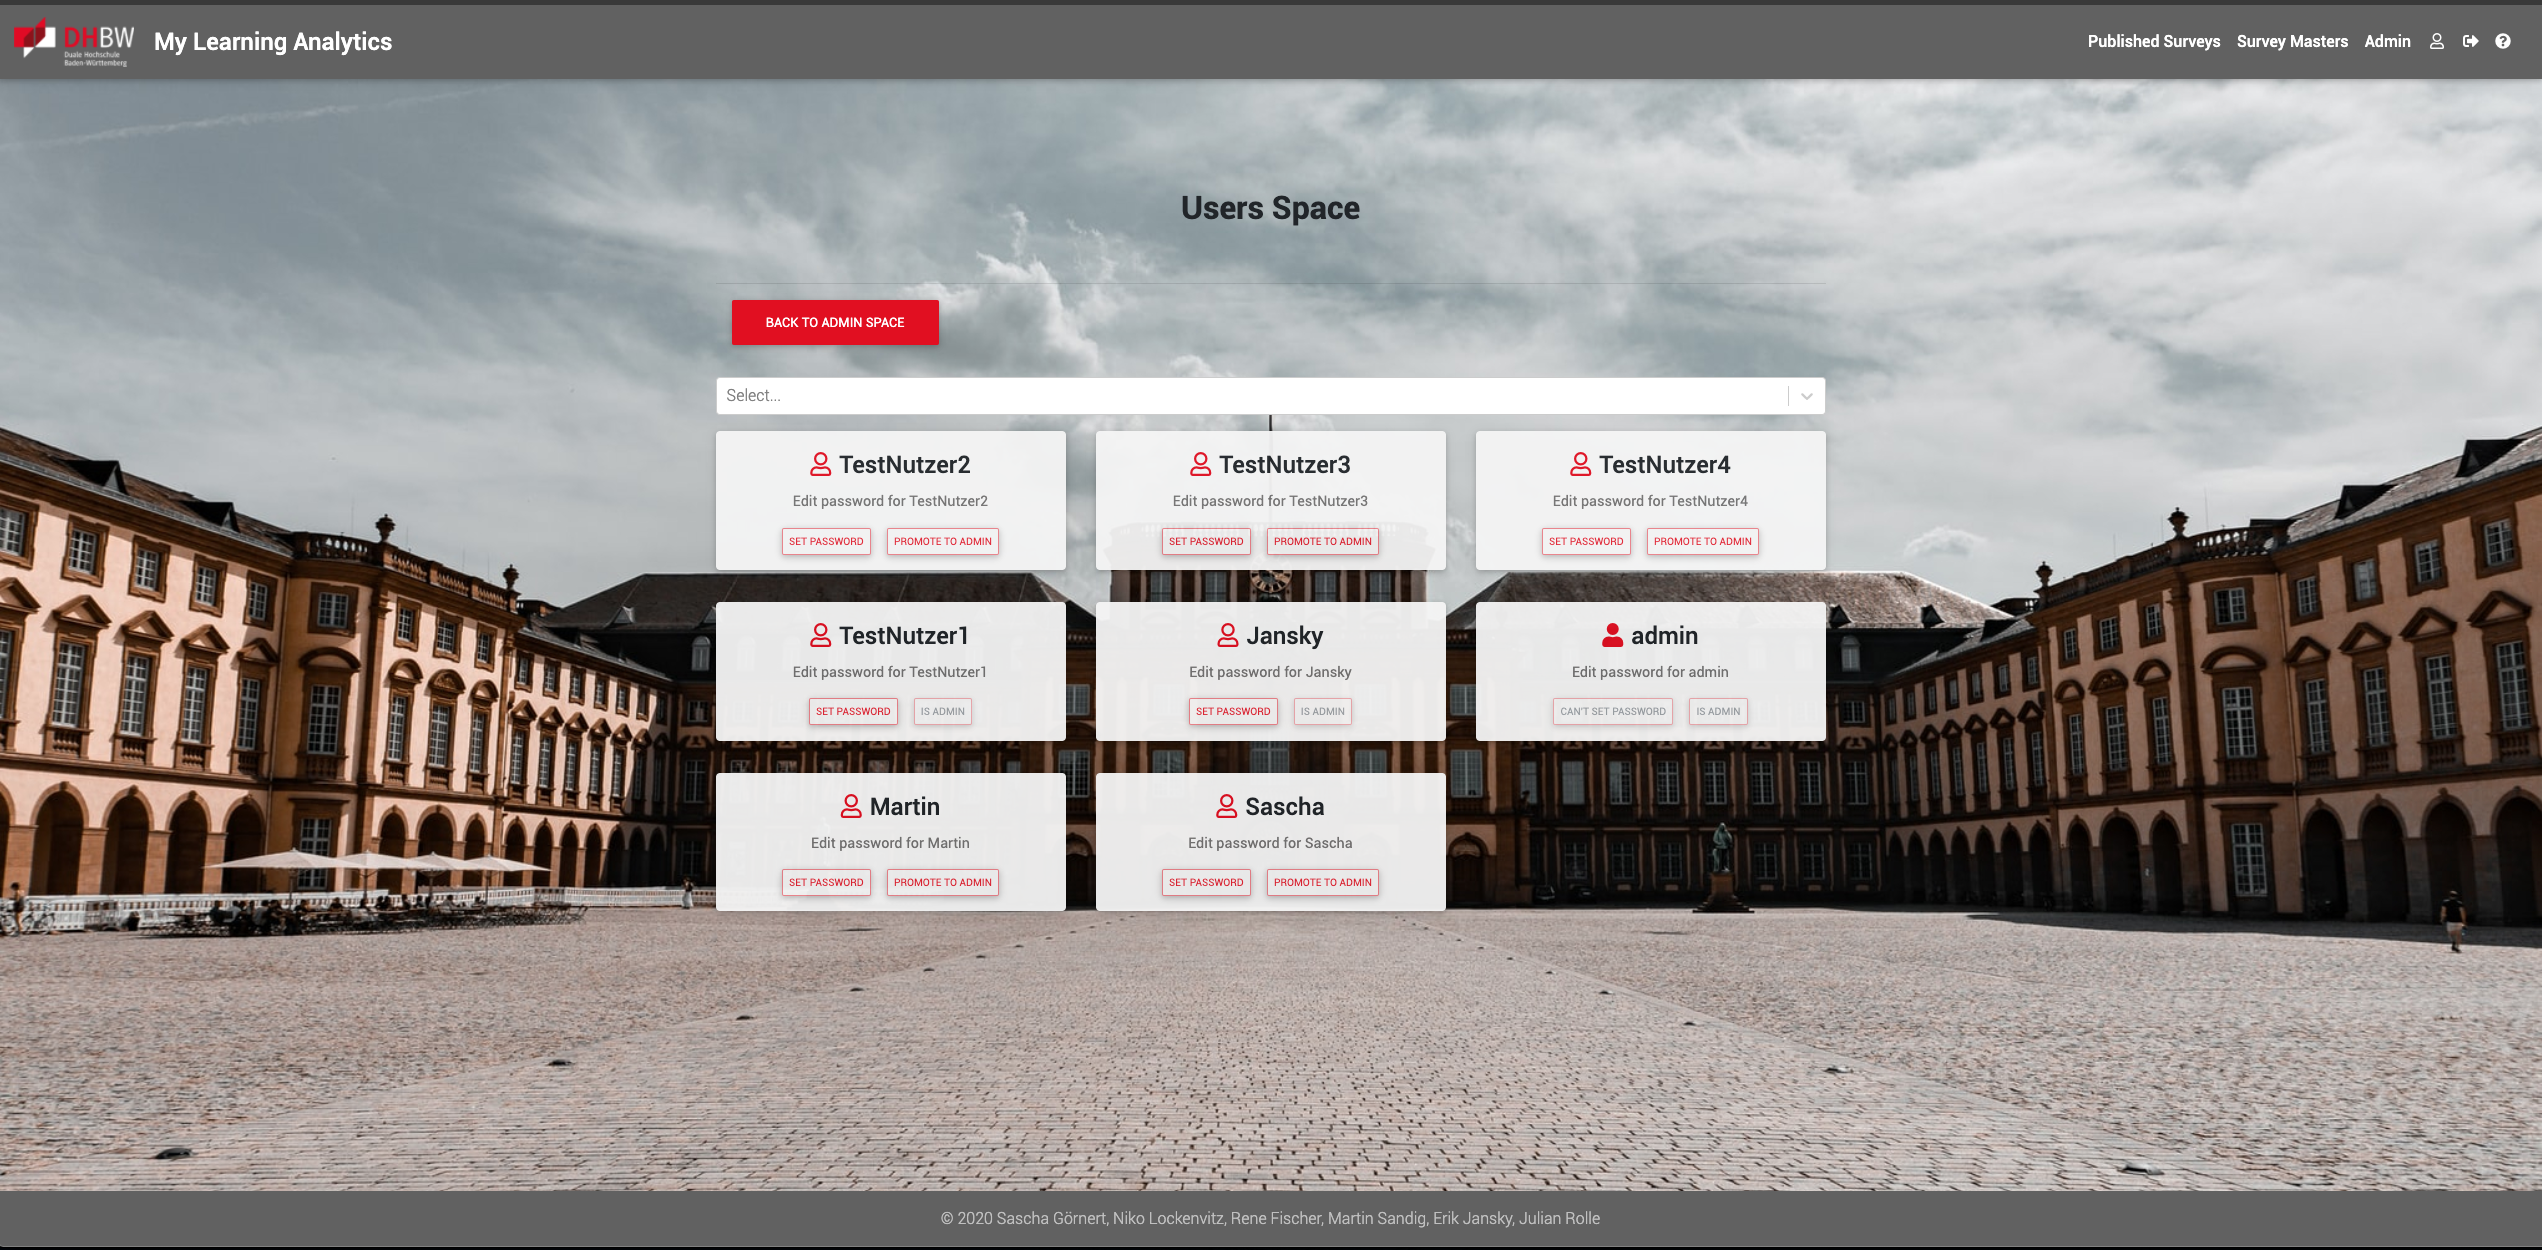
\includegraphics[width=0.95\textwidth, keepaspectratio]{img/client/AdminShowUsers.png}
	\captionsetup{justification=centering, format=plain}
	\caption[\acf{UI}: Alle Benutzer der Anwendung anzeigen]{\acf{UI}: Alle Benutzer der Anwendung anzeigen \\ \quelleScreenshot}
	\label{fig:AdminShowUsersImplement}
\end{figure}

Bei dem Card-Design wurde wert daraufgelegt, dass der Benutzer, der gerade angemeldet ist, farblich anders dargestellt wird. 
Dieser wird als \faUser\xspace dargestellt, wohingegen andere Benutzer nur das Icon \faUser[regular]\xspace (Silhouette) haben. \newline
Das es vergleichsweise oft vorkommt, dass Benutzer ihr Passwort vergessen, wurde hier das Feature des neuen Setzens des Passworts des Benutzers implementiert. 
Dies geschieht über den Button \jinline|Set Password|. \abb \vref{fig:AdminSetNewPasswordImplement} stellt das neue Setzen des Passworts über ein Popup dar.

\begin{figure}[hp]
	\centering
	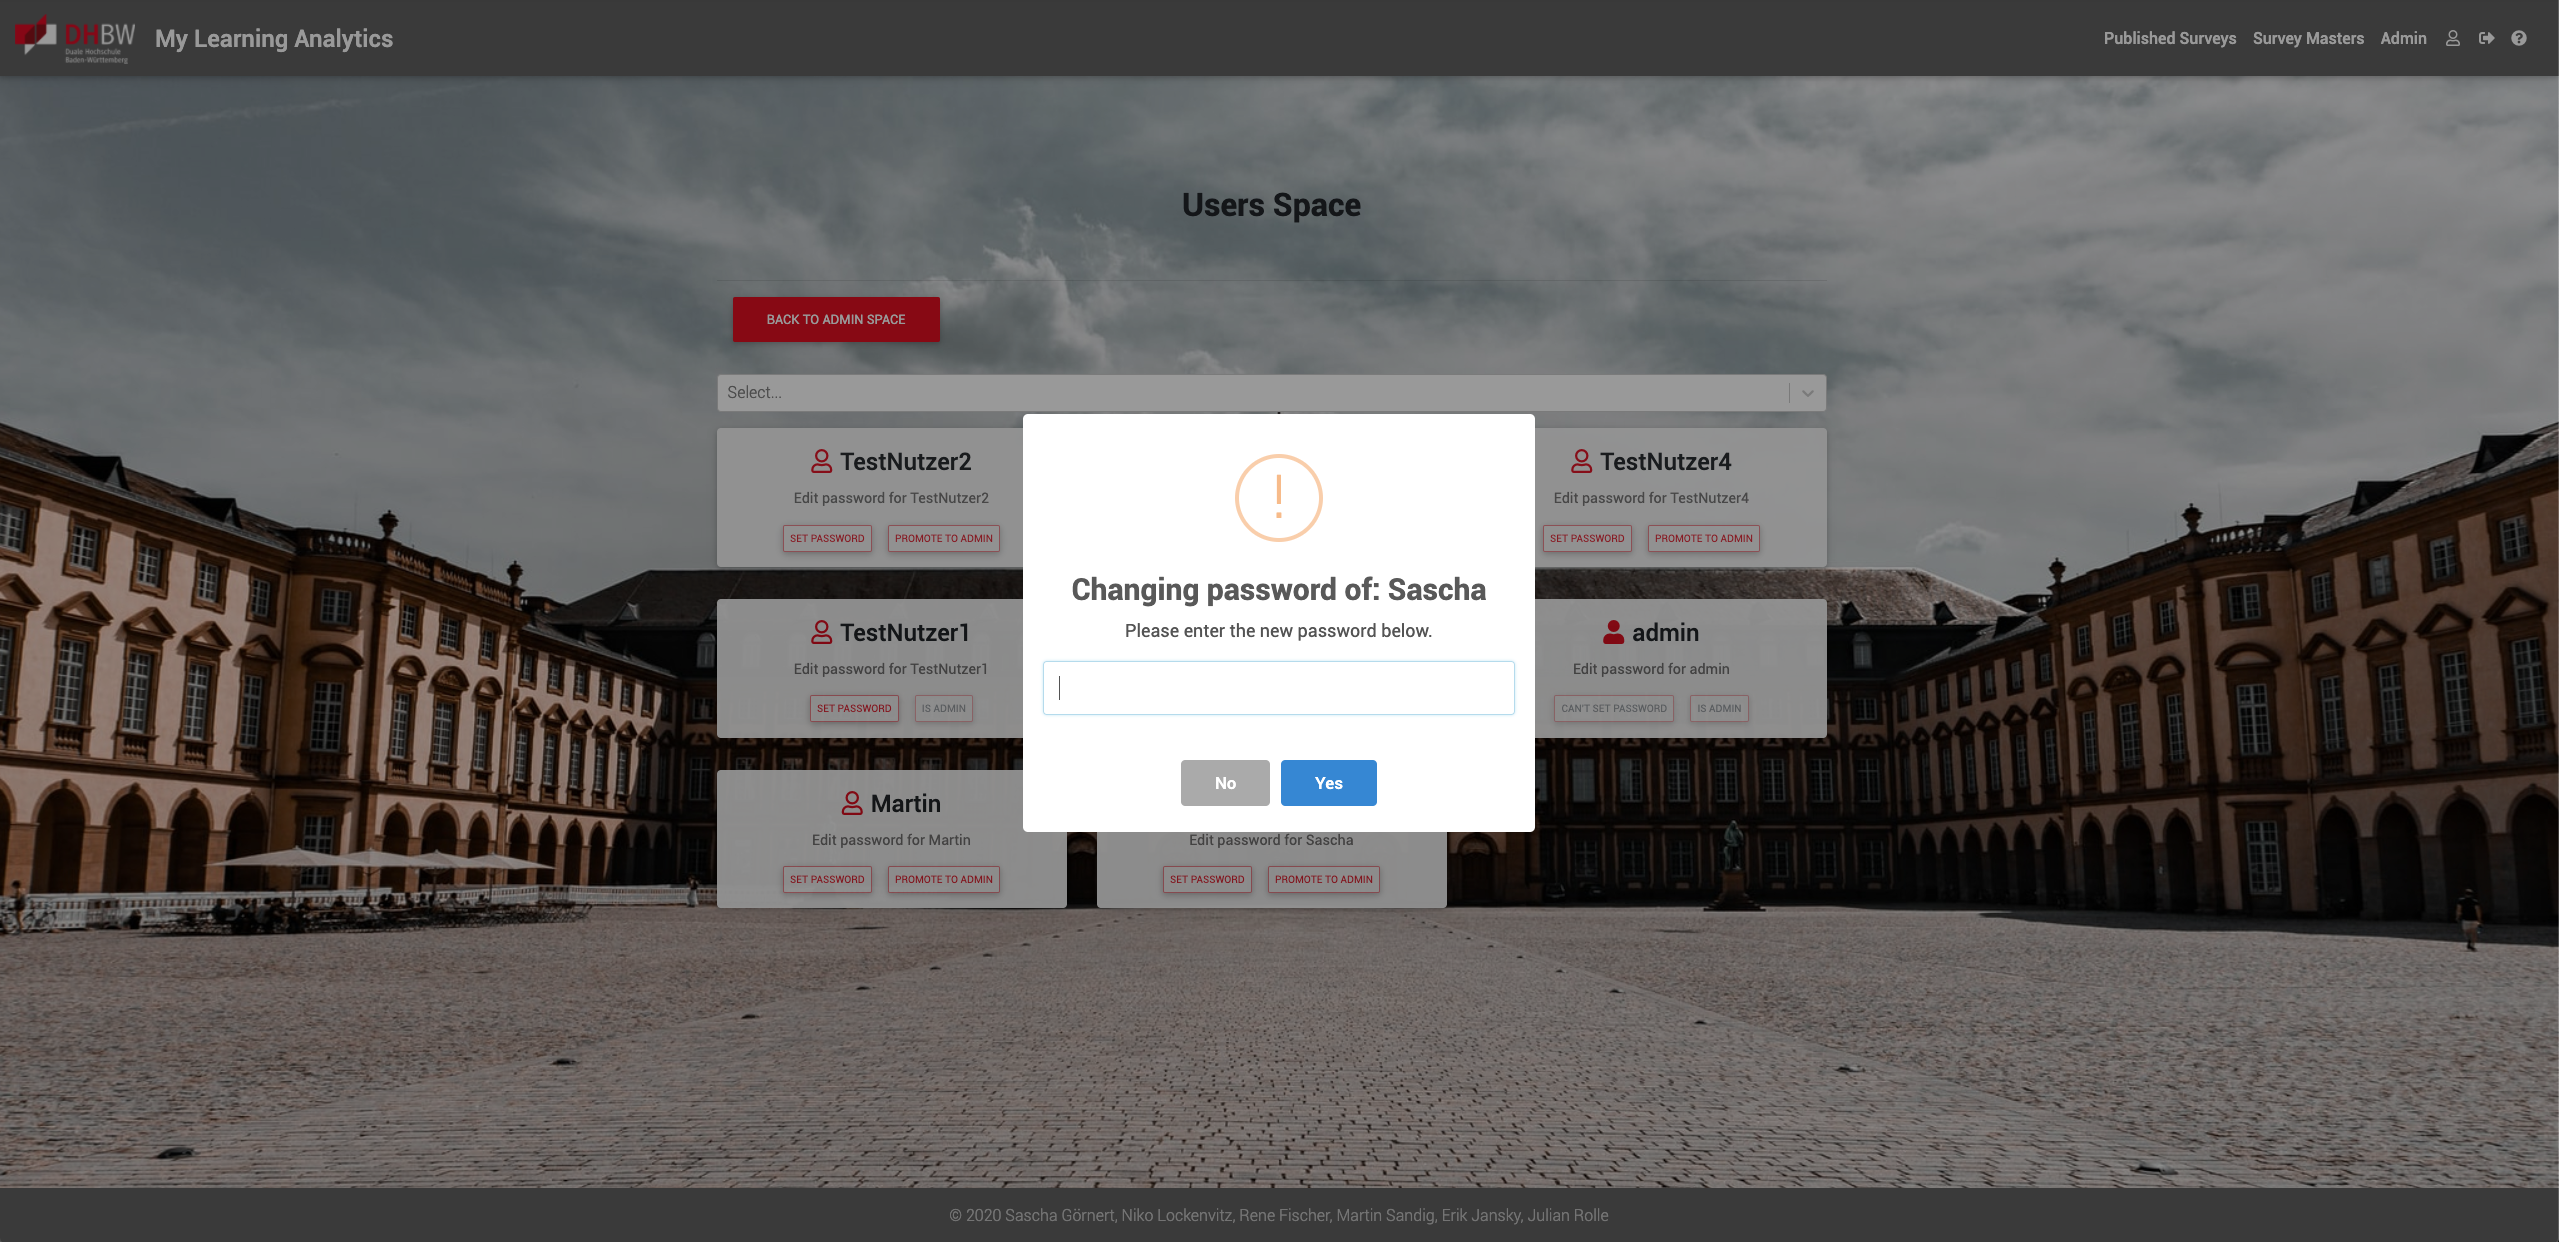
\includegraphics[width=0.95\textwidth, keepaspectratio]{img/client/AdmiSetPasswordOfUser.png}
	\captionsetup{justification=centering, format=plain}
	\caption[\acf{UI}: Setzen eines neuen Passworts]{\acf{UI}: Setzen eines neuen Passworts \\ \quelleScreenshot}
	\label{fig:AdminSetNewPasswordImplement}
\end{figure}

Ein weiteres Feature der Anwendung ist das Ernennen eines Benutzer zum Administrator. 
Hierzu muss der angemeldete Administrator den Button \jinline|Promote To Admin|, wie in \abb \vref{fig:AdminPromoteToAdminImplement} dargestellt, drücken. 
Hat sich der Administrator aus versehen falsch geklickt, wird dies durch eine \emph{Dialog} abgefangen. 
In diesem Dialog wird ihm nochmal seine Aktion, die er durchführen möchte, hingewiesen. 
Er muss mit \jinline|Yes| oder \jinline|No| antworten. 
Um einen \enquote{Trott} des \jinline|Yes|-Buttons bei einem Benutzer zu verhindern, wurde extra die Buttons vertauscht (siehe Abb. \vref{fig:AdminPromoteToAdminImplement}).\newline
Wird der Dialog mit \jinline|Yes| beantwortet, so wird dies nach Rückmeldung der Datenbank sofort angezeigt. 
Der Button \jinline|Promote To Admin| gibt es nicht mehr. 
Dieser ist nun zu Button \jinline|Is Admin| gewechselt.

\begin{figure}[hp]
	\centering
	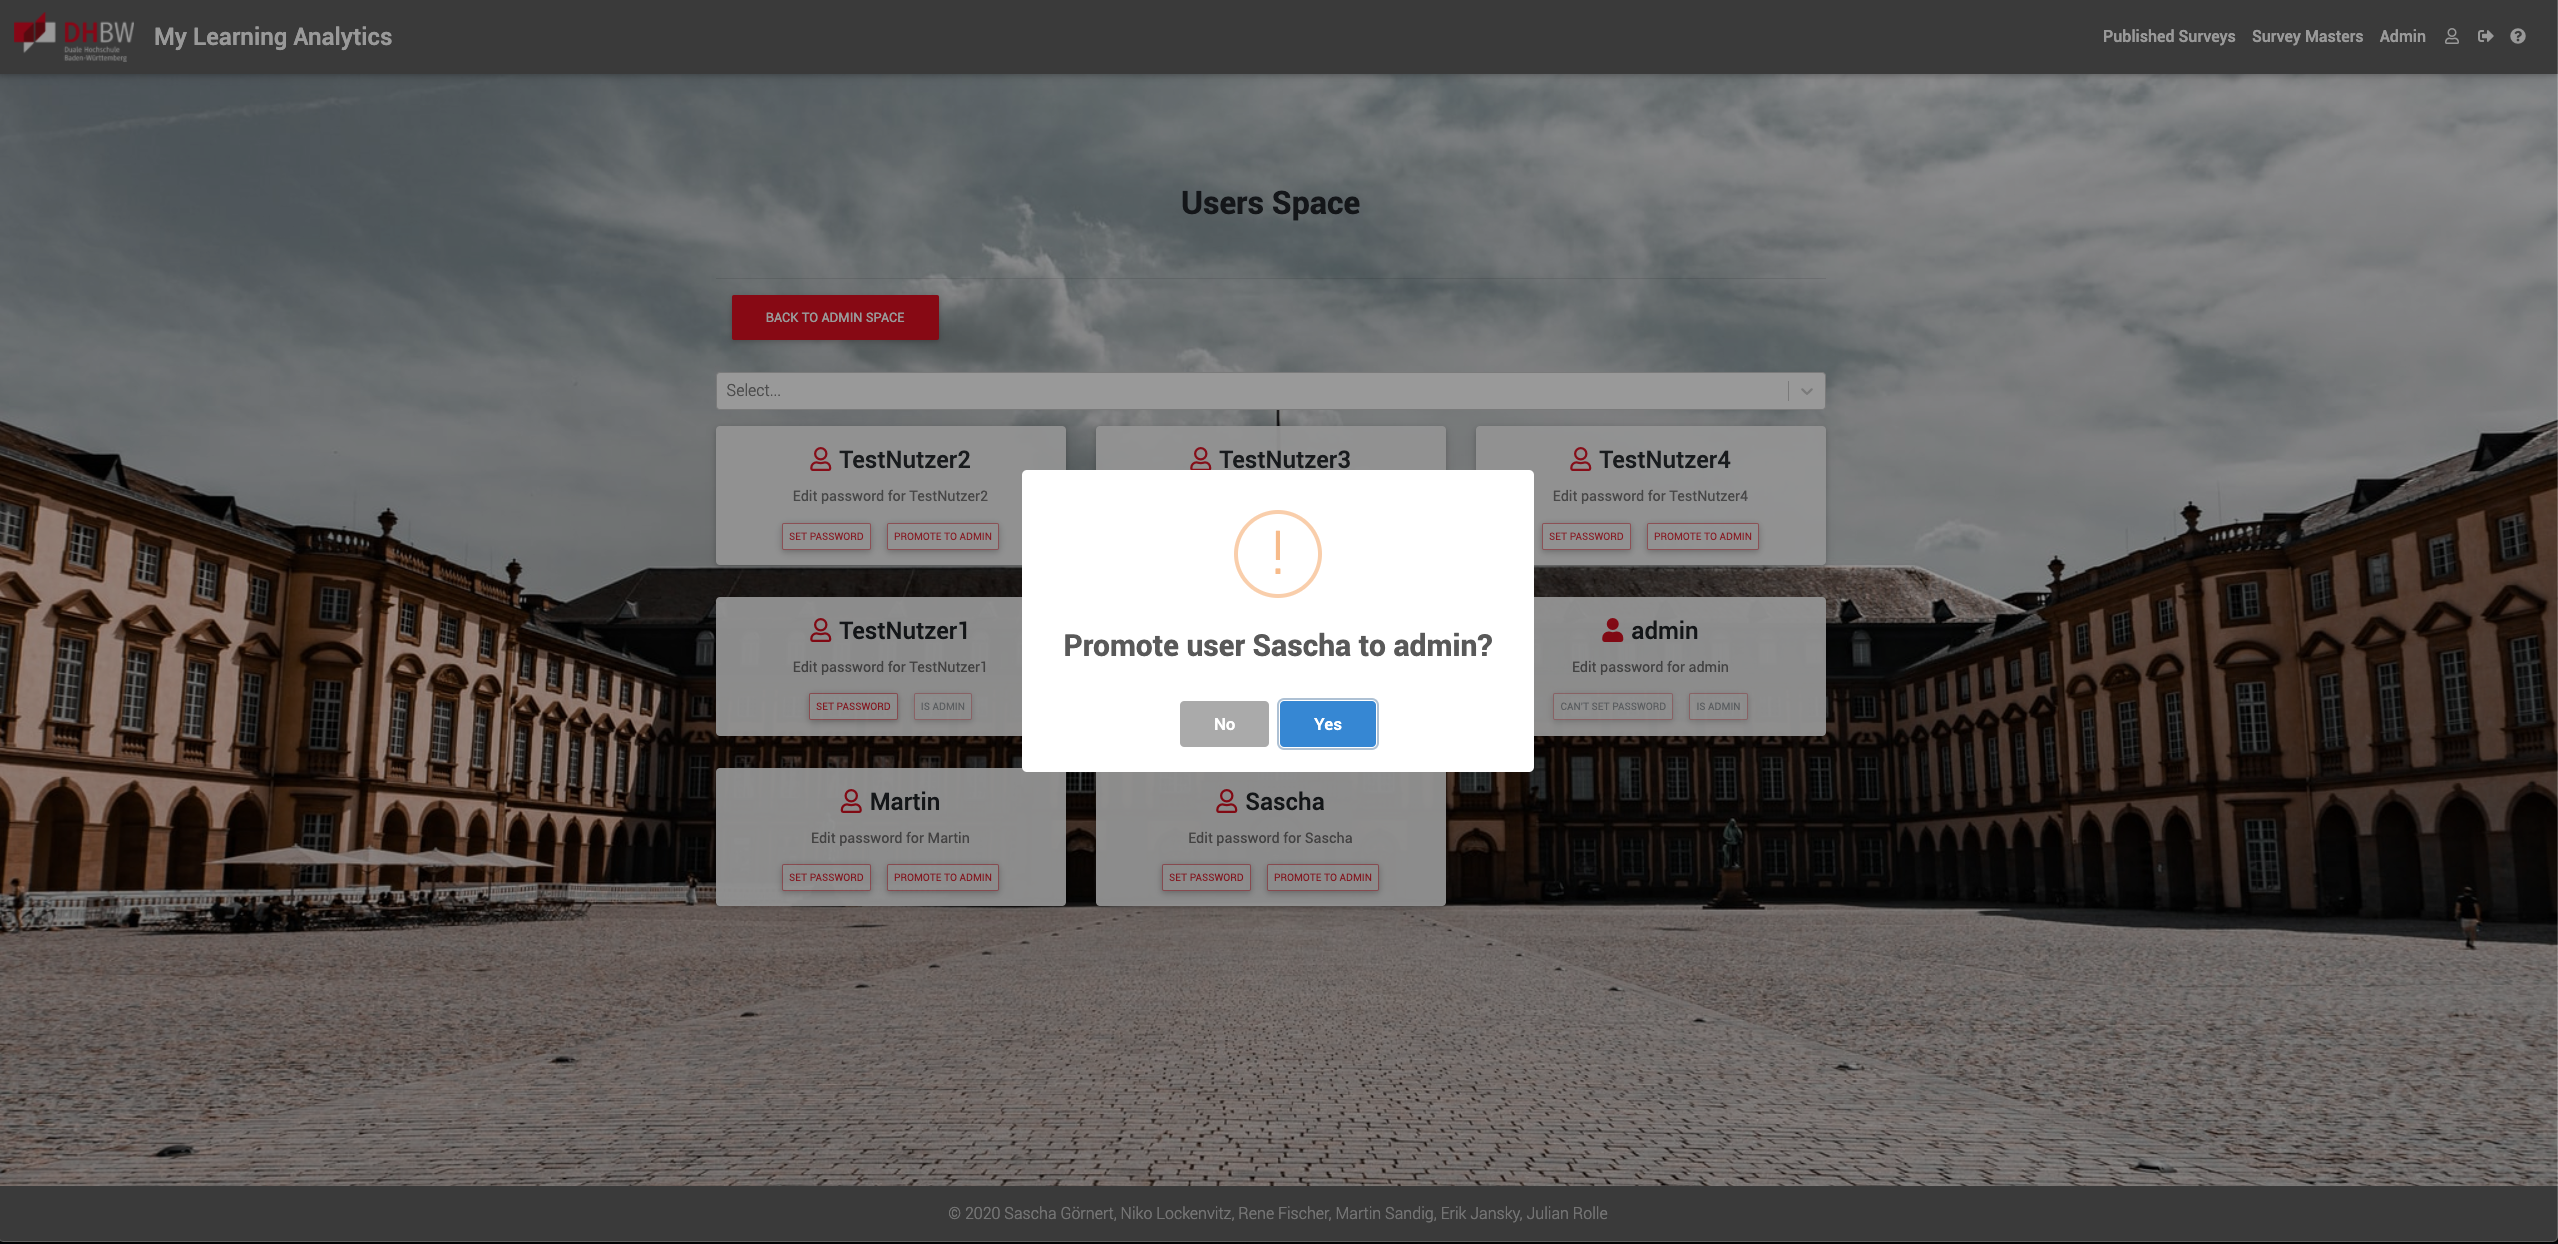
\includegraphics[width=0.95\textwidth, keepaspectratio]{img/client/AdminPromoteToAdmin.png}
	\captionsetup{justification=centering, format=plain}
	\caption[\acf{UI}: Benutzer zum Administrator ernennen]{\acf{UI}: Benutzer zum Administrator ernennen \\ \quelleScreenshot}
	\label{fig:AdminPromoteToAdminImplement}
\end{figure}



